\documentclass[12pt]{article}
\usepackage{float}
\usepackage{caption}
\usepackage{times}
\usepackage{natbib}
\usepackage{graphicx}
\usepackage[section]{placeins}
\usepackage{indentfirst}
\usepackage{fancyhdr}
\usepackage{xcolor}

\usepackage{listings}
\usepackage{color}
\usepackage[hyphens,spaces,obeyspaces]{url}
\usepackage{hyperref}

\hypersetup{
    colorlinks=true,
    linkcolor=blue,
    urlcolor=blue,
    linktoc=all
}

\pagestyle{fancy}
\fancyhf{}
\rhead{\textit{\color{gray}\today}}
\lhead{\textit{\color{gray}C++14 Software Transactional Memory}}
\rfoot{Page \thepage}
\lfoot{\color{gray}\LaTeX}


\begin{document}

\begin{titlepage}
	\begin{center}
	\line(1,0){350}\\
	[0.3 cm]
	\huge{\textbf{Software Transactional Memory\\[0.3 cm]C++14 STM\\ }} 
	\line(1,0){200}\\
	[0.3 cm]
	\huge{\textbf{Research Manual }} 
		\begin{LARGE}
		\\[0.3 cm]Zoltan Fuzesi\\
		\today
		\end{LARGE}
		
		\begin{LARGE}
		\line(1,0){150}\\
		[1.0 cm]
\begin{figure}[h!]
\centering

\includegraphics[scale=0.7]{Pictures/carlow.png}
\end{figure}
	
		
		Software Engineering\\
		Student ID: C00197361\\
		Supervisor: Joseph Kehoe\\
		IT Carlow
		\end{LARGE}
		
	\end{center}
\end{titlepage}

\tableofcontents

\clearpage
\section{Abstract}
The purpose of this research document is to find all the answers associated with the Software Transactional Memory(STM) implementation in C++ programming language. Discover the language syntaxes for transactional statements, how other STM libraries are implemented and what kind of algorithms or logic  should be used in the Software Transactional Memory library implementation. This paper examines the way of replacing the locks with software based transactions using C++14 programming language features.

\section{Introduction}
The Software Transactional memory is a promising alternative to the concurrency control in shared memory systems. Why do we need the STM solution if we can control the concurrent programming with mutex and semaphore. If the Transaction memory has been solved in the Hardware level why it is important to implement at software level as well. What is the difference between the diverse versions of C++ languages. Which is the best IDE and compiler to implement the STM library in C++ language.\\

The aim of this project to create a C++ Software Transactional memory library to control concurrent programming features without locks. Software Transactional memory is a software solution for concurrency control in shared memory access. It provides lock free solution for threaded programming which reduces the challenges in concurrent programming. STM use Transactions to realize automatic conflicts resolution through atomic transactions and avoid the classical lock based associated problems like deadlock and livelock.\\

The research paper contains several sections to describe the main questions around the STM implementation.The first section begins with the concurrent and parallel concepts, such as why we need it and what is the problem with it. What is the difference between concurrent and parallel programming. What is the problem with concurrent programming and how to control the threads in concurrent programming environment.\\

The next section discusses the STM concepts and how it works. Discover the benefits and the problems associated with the software level transactional memory, give sample code for atomic transaction and describe the logical solution, what I need to implement in the project.\\

The following section describes some of the previous STM library implementations in different programming languages with very short explanation.\\

The C++14/17 section will mostly list the differences between the two versions of C++ release and the C++17 version libraries.\\

The last section discusses the difference between the most popular Integrated Development Environment(IDE) functionalities and the available compilers to the  different platforms. This section helps me to choose the best IDE and the compiler version to create the STM library.    


\section{Concurrency}
\subsection{What is concurrency}    
Concurrency in the real-world example could be when many things are happening at the same time simultaneously with someone, example eating the breakfast, reading the newspaper, listening to music and typing text messages. In computer science concurrency is a stage of system/process where multiple processes are executing at the same time and may or may not sharing resources and communicating with each other. The concurrency in a system program required parallel processing, but the challenge with concurrent programming, that the running processes on the processor is running sequentially. To achieve concurrent processing, the process need to split into multiple smaller processes, and running them concurrently. On the modern computers where is more core available inside the CPU (Central Processing Unit) and the programming module not using concurrent programming features the processes can run parallel at same time on the different cores, but those processes are completely independent and not sharing resources.\\ 

To execute a process on the CPU cores concurrently/parallel at the same time, that requires threaded programming. On a single core processor never able to get true concurrency, but true concurrency with threaded programming can happen on multi-core processors.\textit{\color{gray}Figure 1.}

\begin{figure}[h!]
\centering
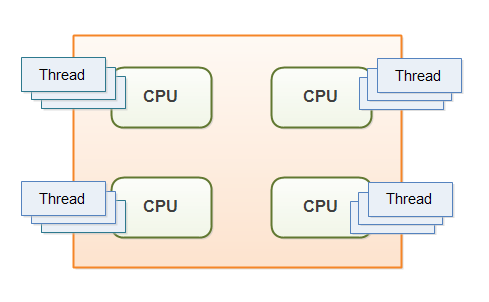
\includegraphics[scale=0.5]{Pictures/Concurrency_multicore-multithreada.png}
\caption{\textit{\color{gray}Concurrency multicore-multithread \cite{Jakob}}}
\end{figure}

\subsection{Why need concurrency}
Moore’s law, is the number of transistors in an integrated circuit doubles approximately every 18 to 24 months. Today’s processors have hundreds of millions transistor embedded into the silicon chip. The Moore’s law held true until around 2005, since the silicon chips are nearly reached the maximum number of transistors of the physical nature of processor material. Actually, the development of silicon chips is ran into a problem with the brick wall. This brick wall is when the size of the transistors are shrinking, but couldn’t scale down the power consumption and the heat any more. So, instead to add more transistors, found the better solution what is to add more execution unit(cores) into the CPU (central processing unit). The more cores can take more instructions at the same time in parallel manner, but the sequential programming or single threaded application perform the same no matter how many cores has the CPU. The parallel, concurrent/multi-threaded programming design is a way to split the process to multiple smaller processes and run then parallel on the CPU cores, that offers much better throughput to the CPU.\cite{Vasudevan}


\subsection{Single-core, Multi-core}
Back in days the computers had only one core in the CPU, and all the processes, running programs were executed sequentially on the single-core CPU one by one with various execution time, depends on the operating system queue logic. In other world, when more than one process/program were executed on the single core system, those processes needed to wait in the queue while executed sequentially on the same core on the CPU. The process can run concurrent on a single-core processor, but the threads are accessing the process resources different time due the core limitation. True concurrency cannot happen without multi-core system. \textit{\color{gray}Figure 2-3.}\\ 

\begin{figure}[h!]
  \centering
  \begin{minipage}[h!]{0.4\textwidth}
    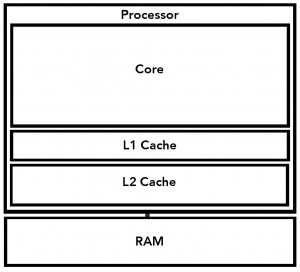
\includegraphics[width=\textwidth]{Pictures/single_core.png}
    \caption{\textit{\color{gray}Single-core CPU.\cite{Looper}}}
  \end{minipage}
  \hfill
  \begin{minipage}[h!]{0.4\textwidth}
    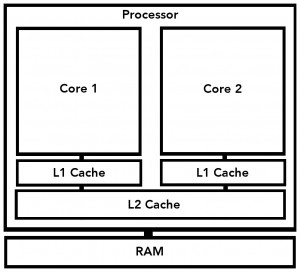
\includegraphics[width=\textwidth]{Pictures/multi_core.png}
    \caption{\textit{\color{gray}Multi-core CPU.\cite{Looper}}}
  \end{minipage}
\end{figure}

On the modern computers the CPU has more than one core, the processes can run parallel on the different cores at the same time. So, if multiple processes running on the operating system, those processes can be executing same time on the same processor on different cores. With these changes of the CPU architecture the parallel computing has been achieved but the single processes still running sequentially on the separated cores inside the processor without threaded programming. Therefore, the true concurrency is the parallel execution on the different cores at the same time, with diverse threads form the same process.

\subsection{Parallel vs. Concurrent}
The parallel computing is executing multiple processes simultaneously on separated cores, while concurrent computing is composing independent processes working together. 

\begin{figure}[h!]
\centering
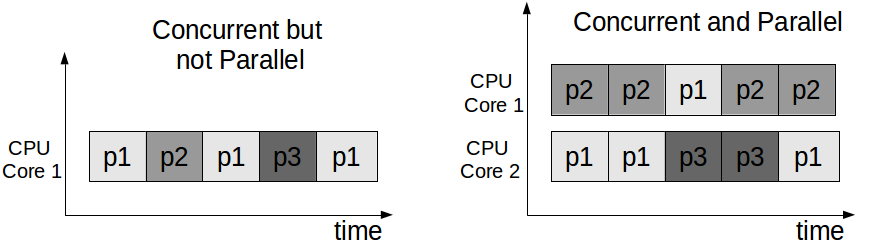
\includegraphics[scale=0.3]{Pictures/concurrent_vs_parallel.png}
\caption{\textit{\color{gray}Concurrent vs. Concurrent and Parallel \cite{Nikolay}}}
\end{figure}

Concurrent computing can happen on single core processor, however if programming design apply threaded programming, that can’t help to run process faster on single core. The process with threaded programming design can run faster on multi-core, since the different processes and the multiple threads can run parallel on multiple cores. \textit{\color{gray}Figure 4.}\\

\subsection{Process vs. Thread}
Process (heavy-weight) is a running instance single thread of program in execution. Each process has its own address space in the memory, that is not shared between the running processes. If two processes need to communicate, they must use IPC (Inter process communication) which allows processes to communicate and synchronize their actions. This Inter Process Communication happen through the OS (operating system). There are two types of communications such as message passing and shared memory. The OS controlling how to use the shared memory and use lock to close out the other process while the another read or write the memory space. The other way for communication between processes is the message passing, where pipe created between the processes and use consumer-producer synchronization. To create processes can be expensive, as each process has its own address space, program code, file handles.\\

\begin{figure}[h!]
\centering
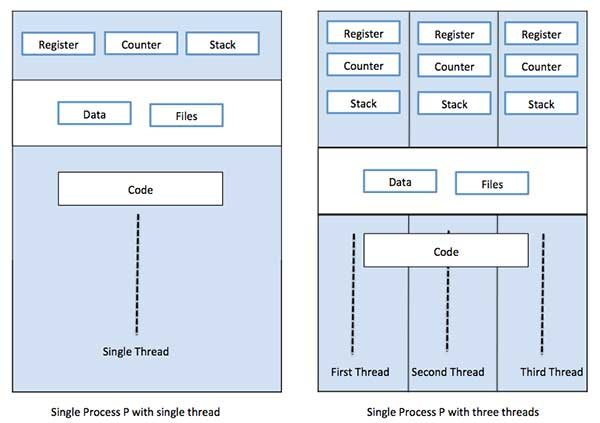
\includegraphics[scale=0.5]{Pictures/single_multi_thread.png}
\caption{\textit{\color{gray}Process vs. Multiple Threads \cite{Nikolay}}}
\end{figure}

Thread is a Light-weight process(LWP). Using threads is a way to improve the performance of the process (running application) through parallelism and concurrency. When the program executed and the instruction-set loaded into the memory, then the process has created. Using concurrent programming design, to create any number of threads associated with the process to run concurrently, parallel on the CPU cores. Those threads are belonging to the same process and sharing the same memory space. Because the threads are sharing the same memory space, therefore use of shared resources leading to new way of resource control. This resource control derives to new issues that requires reliable techniques to synchronize their actions, execution, memory allocation and scheduling time.\cite{Tutorialspoint}\\\textit{\color{gray}Figure 5.}\\\\
 
\subsection{Issues}
The multi-threaded programming use parallel and concurrent programming design, that derives to new issues and require creating locks on shared variables/memory spaces. The unsynchronized shared memory access introduces to race conditions. Race condition is when more than one thread try to access the shared memory space and try to read and write the memory at the same time. If the race condition is not controlled and the threads accessing and modifying the memory at the same time, that cause unexpected behaviour of the process.\textit{\color{gray}Figure 6.}

\begin{figure}[h!]
  \centering
  \begin{minipage}[h!]{0.4\textwidth}
    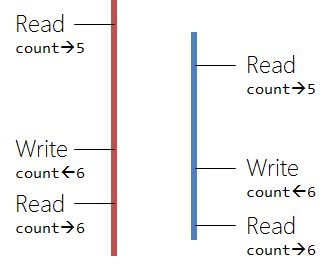
\includegraphics[width=\textwidth]{Pictures/issue1.png}
    \caption{\textit{\color{gray}Unsynchronized\cite{Tutorialspoint}.}}
  \end{minipage}
  \hfill
  \begin{minipage}[h!]{0.4\textwidth}
    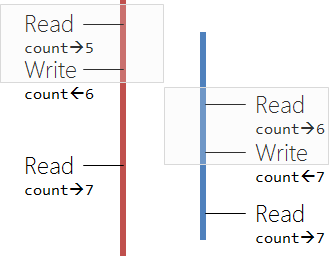
\includegraphics[width=\textwidth]{Pictures/issue2.png}
    \caption{\textit{\color{gray}Synchronized\cite{Florian}.}}
  \end{minipage}
\end{figure}

To solve race condition, in concurrent programming design must use mutex and semaphores to control the shared memory space/shared variables access by the multiple threads.

	\subsubsection{Mutual Exclusion and Semaphores}
Mutex is a mutual exclusive flag. Mutual exclusion is a type of gate that is ensuring to reduce accessibility to a shared resource to only one thread at the same time. The other solution is to use Semaphores. Semaphores is somewhat like an integer value and can do only two operations on it, increment and decrement. Those two operations can happen through methods like Signal and Wait. If the value of the Semaphore is zero, then other threads cannot be pass the line where the method call happened.\citep{Nick&Julie}
So, mutual exclusion and Semaphores can solve the race conditions problem, but may lead to other problems like Deadlock - Live lock and Starvation.

	\subsubsection{Dedalock}
Deadlock is a condition, when two threads try to access the same shared resource and waiting for each other to do some action. Deadlock often arises because the control of semaphore or mutex applied logically wrong way to protect the critical section to access by more than one thread at the same time.\textit{\color{gray}Figure 8.}

\begin{figure}[h!]
\centering
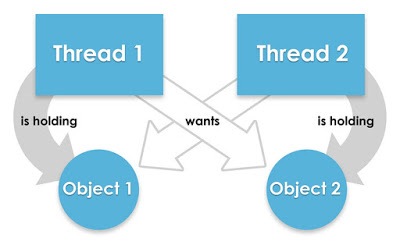
\includegraphics[scale=0.5]{Pictures/deadlock.png}
\caption{\textit{\color{gray}Deadlock \cite{Paul}.}}
\end{figure}

	\subsubsection{Live-lock}
Live-lock is a  situation when two threads are repeatedly access the critical section and the program detect the deadlock situation and release the lock to the other thread. After, both threads are trying to access the critical section and release again, but no progress being made, hence the name is Livelock. \textit{\color{gray}Figure 9.}

\begin{figure}[h!]
\centering
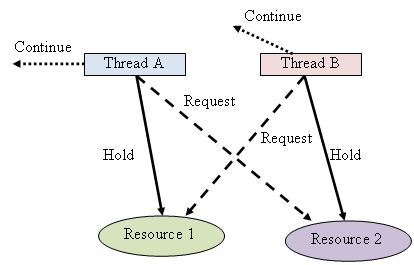
\includegraphics[scale=0.5]{Pictures/livelock.png}
\caption{\textit{\color{gray}Livelock situation \cite{installsetupconfig}.}}
\end{figure}

	\subsubsection{Starvation}
Starvation is the state when some threads are making progress, but other threads are waiting in the queue for execution. The waiting thread priority can be to low and never will get out of the queue to make progress.\textit{\color{gray}Figure 10.}

\begin{figure}[h!]
\centering
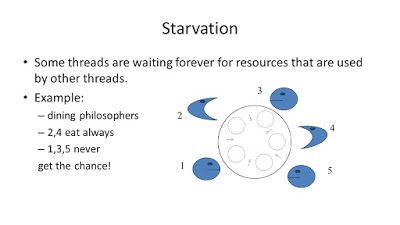
\includegraphics[scale=0.6]{Pictures/starvation.jpg}
\caption{\textit{\color{gray}Starvation \cite{Sitansu}.}}
\end{figure}
\clearpage
\subsection{Concurrency Conclusion}
There are advantages and disadvantages of concurrent and parallel programming pattern. With concurrent and parallel programming the applications are able to handling multitasking within the application. While the user interacting with the user interface, the program able to perform other tasks in the background. For instance, the web browser able to render high number of web pages and the browser tabs at the same time perform number of downloads in the background.  

	\subsubsection{Advantages}
{\setlength{\parindent}{0cm}
The main advantages of the concurrent/multi-threaded application are:\\

Performance:\\
The processes in which executed with multi-threaded technique can reduce the computation time and resolve problem in faster manner.\\

Reactive:\\
The single program able to run multitasking in the background while user keep interacting with the application(multitasking).\\

Maximum CPU throughput:\\
Parallel concurrent programming design only way to exploit the multi-core CPU in efficient manner. \\

High performance:\\
While single threaded application performs the same no matter how many cores in the CPU, the concurrent application uses all the cores in the CPU.}
	\subsubsection{Disadvantages}
{\setlength{\parindent}{0cm}
The main disadvantages of the concurrent/multi-threaded application are:\\

Difficult to write code:\\
Multi-threaded applications are not easy to write.\\

Debugging:\\
Much harder to regenerate the same error in the multi-threaded application and harder to debug to.}

\clearpage
\section{Software Transactional Memory (STM)}
\textit{"Software Transactional Memory (STM) is a mechanism that allows transactions on memory similar to database transactions."}\cite{Haskell}
STM is a concurrency control for threaded programming, that does not use locks and semaphores as its primary locking mechanism. However, concurrent programming with loks and semaphores solving the issues to access shared memory space by more than one thread at the same time, but it is still very complicate to write efficient programs by the programmers specially if the software is working in big scale.\\

Software Transactional memory use transaction instead of locks and semaphores, that is similar to the database systems. The main purpose of STM to avoid concurrent programming issues and guaranties safety operations on shared memory space.\cite{Kasper}\\

The hardware support for STM is the Hardware Transactional memory(HTM).
A Hardware Transactional Memory (HTM) system uses multi-word(multi-fixed size piece of data) synchronization operations of the CPU for threads to manipulating shared data.\\

{\setlength{\parindent}{0cm}
Transactions are very important part of the STM solution.  
There are four properties of the transaction operations, it know as the ACID properties.}
\begin{enumerate}
\item \textbf{Atomic} operations can guaranties that all of the operations happens, or none of them.
\item \textbf{Consistency} all data will be consistent and never get data violated.
\item \textbf{Isolation} all the transactions within the system completely separated and they can not access each other data until not finished. 
\item \textbf{Durability} guaranteed that all the data changes will be recorded after the transaction has finished and available to the other transactions. \textbf{But it is not applies to the Memory Transaction.}
\end{enumerate}

\subsection{Transaction.}
In real life example for transaction is a money transfer between two account in the bank. When someone wants to transfer some amount of money from his/her bank account to an another bank account, the biggest problem is the state of the transferred amount of money. How the system should implement the transaction?  First decrement the source bank account and the increment the destination bank account with the amount was sent. The other solution could be if the target account in incremented and then the source decremented? What's happen with the transferred money if the system goes down during the transaction before the amount arrived to the destination, but the source account decremented already?\\

The solution for those questions is the Transaction. The transaction is a way of processing, where all the separated processes need to succeed, otherwise the transaction will fail. In the bank transfer case, if the destination bank account is not available, then all the processes involved in the transaction will rolling back, and the amount of money goes back to the source bank account.\textit{\color{gray}Figure 9.}\\

\begin{figure}[h!]
\centering
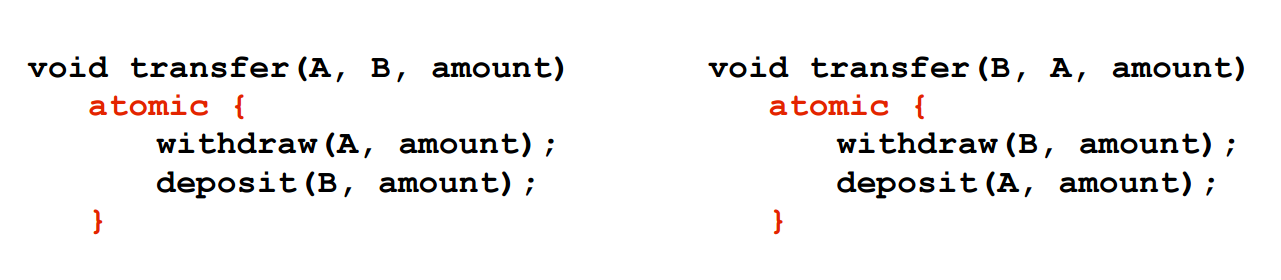
\includegraphics[scale=0.3]{Pictures/realLife.png}
\caption{\textit{\color{gray}Transaction memory \cite{TMvsLock}.}}
\end{figure}

\subsection{Transactional Memory(TM).}
Transaction Memory is an approach of concurrency management and it is called optimistic, because assume multiple transactions can complete frequently without interfering with each other. Transactional Memory is a synchronization for the threaded/multi-core programming to simplify concurrent programming to avoid of the concurrent programming issues like Deadlock, Race Condition, Corruption, Lost wakeup. The Transactional Memory control provides atomic and isolated execution for region of codes. The abstraction of the atomic transaction required a hardware mechanism, that detect conflicts and revert back all the changes made on the shared memory space.\\

When any thread enters the block of code that is use atomic execution, the other threads can't access or see any modification until the thread is not finished with the code execution and leave the block. This software design can avoid of unnecessary concurrent programming conflicts and the shared variables overwriting issues. \cite{BDJ}\\


The concurrency control mechanism analogous to the database transactions that controls the access to the shared memory in concurrent programming. The STM functions are alternative to the lock-based synchronization mechanism, but it is implemented in a lock-free way. The transaction is when a block of code executes series of actions on the shared memory space. \citep{STM} While database transaction as a result are written to the disk, until Software Transactional Memory has a life-time while the code executing and only change the state of the shared variable by the threads in the memory.\textit{\color{gray}Figure 12.}

\begin{figure}[h!]
\centering
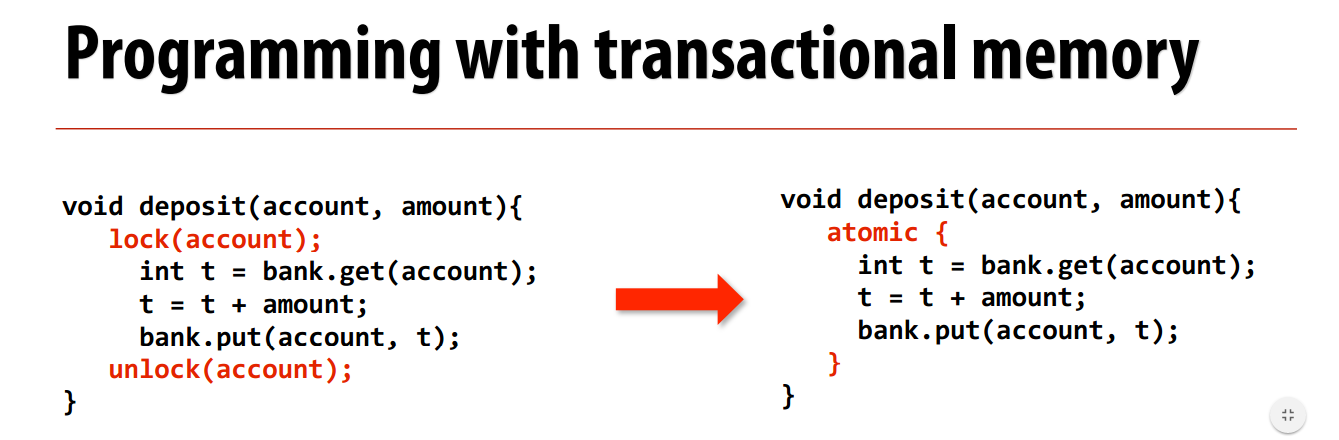
\includegraphics[scale=0.2]{Pictures/lockvsatomicjpg.png}
\caption{\textit{\color{gray}Transaction memory \cite{TMvsLock}.}}
\end{figure}



\subsubsection{How does it work?}
The Transactional Memory software solution allowing the transactions within the process to be executed in parallel and monitoring the access to the shared/transaction variables. Whit this transaction synchronization monitoring solution the software able to detect a conflict between transactions and allowing only one transaction at the same time to access the shared variable and rolling back to the other transactions. So, because the  Transaction Memory is lock free, the threads are not waiting to the lock, all of them can access the atomic block in parallel and make changes on the shared memory space. Increasing the associated version number with the memory block and assuming there is no conflict happens. When the threads are finish with the atomic block execution, they are checking the version number associated with the memory block in which they are working on and if the version number are higher then the version number use by the thread, that is indicates, other threads are made changes on the same memory space. In this case the transaction can not happen and must to restart/roll-back caused by the version number conflict. In this case the thread must roll-back all the changes happened on the variable and restart the transaction. This process will goes on until all the transaction finish they execution and the threads are joining back to the main process. \cite{Stack}\textit{\color{gray}Figure 13.}\\

\begin{figure}[h!]
\centering
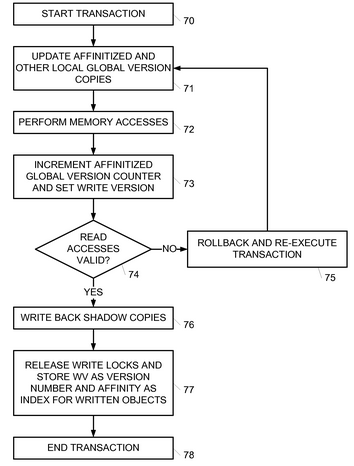
\includegraphics[scale=0.3]{Pictures/rollback.png}
\caption{\textit{\color{gray}Transaction rollback \cite{Patent}.}}
\end{figure}


{\setlength{\parindent}{0cm}
The proper STM implementation at least must has two properties:}
\begin{enumerate}
\item \textbf{Atomic.} Grouped set of generic operation executed on the shared memory space or fail them all.   
\item \textbf{Serializable.} The current state of the data structure can be reconstructed by simply replaying the transaction by sequential order from start to end.\cite{Dennis}
\end{enumerate}

The diagram below shows the single shared data-set space use by two threads. The data can be anything from array, binary tree, hash map etc. However, the data-set shared, but the two threads are accessing different variables in the data-set. Those two variable has a unique memory address, thus the threads can update the variables concurrently.\textit{\color{gray}Figure 14.}\\

\begin{figure}[h!]
\centering
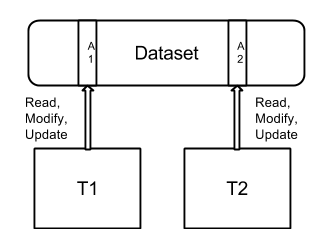
\includegraphics[scale=0.4]{Pictures/STM.png}
\caption{\textit{\color{gray}Shared data-set by two threads. \cite{Dennis}.}}
\end{figure}

The simple illustration of Software Transactional Memory, need at least two thread and those threads must to access the same memory space at the same time to try update the shared variable. \textit{\color{gray}Figure 15.}\\

\begin{figure}[h!]
\centering
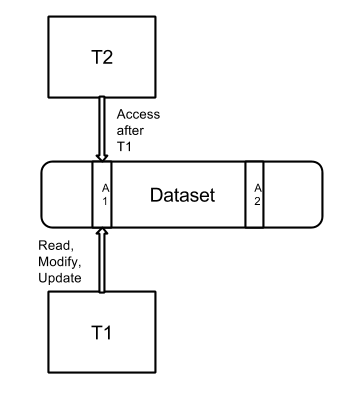
\includegraphics[scale=0.25]{Pictures/STMtwoThreads.png}
\caption{\textit{\color{gray}STM implementation with two threads. \cite{Dennis}.}}
\end{figure}


When the first thread(T1) get ownership of the memory address and the second thread(T2) try to access the same memory space, then the second thread will fail. Because, the software use STM implementation, the method must be use atomic and the second thread keep trying get access to the memory space. When the first thread(T1) finish it is action with the shared variable, then releasing the memory space and the second thread(T2) can execute the it's transaction on the shared variable.\cite{Dennis} \\


{\setlength{\parindent}{0cm}
All updates occur via transactions:\cite{Kenneth}\textit{\color{gray}Figure 16.}}
\begin{enumerate}
\item If only transaction A is updating identity B, no locks are encountered.   
\item If transactions A and B are updating identity C at the same time
\item The first thread get access to memory space and the others are rolled back and retried.
\end{enumerate}

\begin{figure}[h!]
\centering
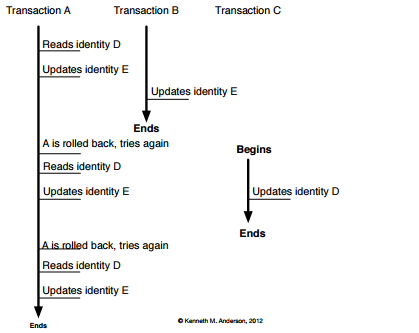
\includegraphics[scale=0.8]{Pictures/STMRollback.png}
\caption{\textit{\color{gray}STM rolling back atomic function. \cite{Kenneth}.}}
\end{figure}

\subsection{STM algorithms}
\subsubsection{Lock based concurrency}
Is a mechanism to control threads to access shared memory space. It uses locks to take control or ownership of the mutex lock before any other thread can access then critical section to make changes on the shared variable. Whit this way of programming design the object is associated with the lock.\cite{Volkmann}\\

{\setlength{\parindent}{0cm}
\textbf{Benefits :} in very small system easier to implement lock based concurrency.\\

\textbf{Issues:} needs explicit control of lock, that can be very difficult in big system. Easy to produce deadlock, livelock.}\\
\subsubsection{Actor based concurrency}
The actor model is an another way to control concurrent programming. In this way the actors are  separate light-weight threads. Instead take ownership of the lock the actors are communicating with each other via message passing.cite{Volkmann}\\

{\setlength{\parindent}{0cm}
\textbf{Benefit :} memory not shared.\\

\textbf{Issues :} Difficult to coordinate actors communication, big messages.}\\
\subsubsection{STM implementation}
One way to avoid of corrupting data in shared memory to provide immutable data structure or collection classes. If data can not changed, then don't need to be protected. This way the program create same data structure in the memory. It can be slow and using lots of memory.\cite{Volkmann}\\

The another option to implement STM algorithm to use time stamp or version number on the transactions. The time stamp or version number is a global progress condition variable that use to compare value at the beginning and at the end of the transaction. The progress condition will be used to determine the commit time or the number of commits by the threads in the transactional processes.\\

When the thread access the transactional function it will check the global version number and store it. At the end of the transaction will compare the stored version number with the global version number. If the stored version number lower then the global one, the transaction aborts and restart. If the version number is same as the global one then it will commit the changes in the shared memory and leave the transactional block and increase the global version number. This process will be continuing until all the threads will finish with it's function in the transactional process.\cite{Timstamp}\\

\subsection{Why use STM?}
Why programmers should use Software Transactional Memory implementation if the semaphores and the mutex are solving the accessibility problem with the shared variables. Because, managing concurrency with locks by the programmers are very difficult. For small, trivial system, managing the locking solution are possible, but scaling that system into more complex that is very difficult and unnecessary.\\

In other worlds the STM try to simplifying the concurrent programming. In threaded programming must use locks and condition variables. With STM easier to write clear code, since don't need to use locks and condition variables and programmer can specify code regions are executing atomically.\\

Locking provides poor support for code compositions and reuse. The software that use transactional programming features, every shared memory access divided into transactions, which are indented to be executed atomically. All the transactions operations are atomically in which all changes takes place or all rolling back if any part of the transactions has failed.\citep{STM}

\subsection{STM Code semantics.}
"\textit{C++ supports transactional memory in two flavours: synchronized blocks and atomic blocks.}\cite{Grimm}
The following are sample codes for atomic and synchronized transactional declaration.\\
In transaction there is no default action, explicit need to tell what should be happen:

{\setlength{\parindent}{0cm}
\subsubsection{Four ways to demarcate a transaction}
Atomic and synchronized -like code region :\cite{Torvald}}
\hfill
\begin{lstlisting}
synchronized
{
	//synchronized block behave as a global block,
	//not rolling back
}
atomic_noexcept
{
	//no exeption inside the block
	//if exception throws std::abort will be called
	//and the program aborts, and roll-back
}
atomic_cancel
{  
	//default std::abort called, but if transaction_safe
	// exception throws the cause transaction to rollback
}
atomic_commit
{
	//if exception occurs cause the transaction to commit
}

transaction-safe exceptions :std::bad_alloc,
std::bad_array_length, std::bad_array_new_length,
std::bad_cast, std::bad_typeid, std::bad_exception,
std::exception,
\end{lstlisting}
{\setlength{\parindent}{0cm}
The synchronized - Allows non-transactional synchronization. It can not cause deadlock because it is not protects the memory block but protects the total program. However, it is not transaction safe.\\
The atomic * - Allows transactional-safe code, and synchronization.\\
The atomic commit - transaction commit everything done so far.\\
The atomic noexeption - Terminates the program with undefined behaviour.\\
The atomic cancel - Will roll back the transaction.
\cite{Torvald}\\

Hello world example .
}
\begin{lstlisting}
void foo()
{
	cout << "Hello World!" << endl;
}
\end{lstlisting}
{\setlength{\parindent}{0cm}
If more then one thread executing the same code block the output can be printed in any order from half printed sentence mixed with the another printed sentence :
\textbf{Hello Hello world!\\
world!}\\

OR\\

\textbf{Hello world!\\
Hello world!}\\

But if the foo function use transaction the output could be like the follow:
}
\begin{lstlisting}
void foo()
{
	cout << "Hello World!" << endl;
}
//Thread 1			//Thread2
atomic_noexcept			atomic_noexcept	
{				{
	foo();				foo();
}				{
\end{lstlisting}
{\setlength{\parindent}{0cm}
The output can be like the follow:\\
\textbf{Hello Hello ... Hello}\\
It could be print more Hello because one of the transaction rolls back and restart the transaction!\\
}

{\setlength{\parindent}{0cm}
The solution for the threaded function to print out the two sentence in the correct way should use the synchronized transaction:\\  
}
\begin{lstlisting}
void foo()
{
	cout << "Hello World!" << endl;
}
//Thread 1			//Thread2
synchronized			synchronized	
{				{
	foo();				foo();
}
\end{lstlisting}
{\setlength{\parindent}{0cm}
The output will be in the following order:\\
\textbf{Hello world!\\
Hello world!}\\\\
The synchronized function solve the problem but it is not able to roll back the transaction.\\

In transactional function should not use any printing statement, because if the transaction rolls back then the function restart and prints again and again until there is no conflict happens in the function. So, only computations should be in the transactional functions!\\

The non-virtual functions can be declared implicitly as a safe function.
}
\begin{lstlisting}
viod foo(){x++;}

atomic_noexcept
{
	foo();
}
\end{lstlisting}
{\setlength{\parindent}{0cm}
Call the foo function is safe after the atomic definition. It can help with the template functions. In this way the template function can be reuse as a safe function.
}
\begin{lstlisting}
template <class T>
void func(int& x, T t)
{
	f(x++);
}
void(*p1)(int)transaction_safe;
atomic_noexcept
{
	func(v, p1);
}
\end{lstlisting}
{\setlength{\parindent}{0cm}
\subsubsection{Transactional syntaxes}
}\cite{Hall}



\begin{lstlisting}
__transaction_relaxed
{
	//statement
}
__transaction_atomic
{
	//statement
} 
__transaction_safe
__transaction_safe_dinamic
__transaction_unsafe
__transaction_cancel


__transaction_callable
__transaction_may_cancel_outer
__transaction_pure

__transaction_safe_dynamic

__transaction_wrap
\end{lstlisting}
{\setlength{\parindent}{0cm}
\textbf{The transaction atomic} - Other execution code can not see intermediate atomic transaction, can be cancelled.\\

\textbf{The transaction relaxed} -  Other execution code can not see intermediate atomic transaction, can not be cancelled.\\

\textbf{The transaction safe}   - Code block is use safe transaction.\\

\textbf{The transaction unsafe} - Code block is not transaction safe.\\

\textbf{The transaction safe dynamic} - The qualifier may only appear in a function declarator that declares a virtual function in a class definition, but it should be declared as transaction safe. If any function that declared synchronized or atomic call the transaction safe dynamic function can cause undefined behaviour.\\

Some of the declaration has no correct documentation.
}\cite{Torvald}

\begin{lstlisting}
__transaction
__transaction_atomic
__transaction_cancel
\end{lstlisting}
{\setlength{\parindent}{0cm}
\textbf{The transaction atomic and transaction relaxed} - Similar to atomic commit and synchronized.\cite{Torvald}\\
}

{\setlength{\parindent}{0cm}
The following sample codes are demonstrating the atomic, transaction safe and synchronized functions.\\
}
\begin{lstlisting}
int function(){
	int x = 0;
	atomic{
		x++;
		return x;
	}
}

int function() transaction_safe{
	x++:
}

void doSomething(){
 _Synchronized {
 value = doSomethingElse();
 }
}
\end{lstlisting}

{\setlength{\parindent}{0cm}
Explicit transaction safe declaration for template class or template calass function:\\\cite{ISO/IEC}
}
\begin{lstlisting}
template<class T>
void f(T) transaction_safe;

template<>
void f(bool); // not transaction-safe
\end{lstlisting}

{\setlength{\parindent}{0cm}
To initialize the variables in c++ as an atomic variable need use the following variable declarations with the variable type and the assignment:
}
\begin{lstlisting}
std::atomic<variable_type>variable_name;
std::atomic_store(&variable_name, value);
\end{lstlisting}
Or can be done in one line assignment:
\begin{lstlisting}
std::atomic<variable_type>variable_name(value);
\end{lstlisting}

{\setlength{\parindent}{0cm}
\subsubsection{ Atomic variables member functions:}
}
\begin{lstlisting}
fetch_add
\end{lstlisting}
Atomically adds the argument to the value stored in the atomic object and obtains the value held previously 
\begin{lstlisting}
fetch_sub 
\end{lstlisting}
Atomically subtracts the argument from the value stored in the atomic object and obtains the value held previously 
\begin{lstlisting}
fetch_and
\end{lstlisting}
Atomically performs bitwise AND between the argument and the value of the atomic object and obtains the value held previously 
\begin{lstlisting}
fetch_or
\end{lstlisting}
Atomically performs bitwise OR between the argument and the value of the atomic object and obtains the value held previously.
\begin{lstlisting}
fetch_xor
\end{lstlisting}
Atomically performs bitwise XOR between the argument and the value of the atomic object and obtains the value held previously.\\


{\setlength{\parindent}{0cm}
\subsubsection{Atomic variables specialized member functions:}
}
\begin{lstlisting}
operator++ //increment
operator-- //decrement
operator+= //add
operator-= //substracts
operator&= //and
operator|= //or
operator^= //xor
variable->store(value) //Modify contained value
variable->load()  //Read contained value
\end{lstlisting}
\subsection{Compiler support.}
To use the Transactional Memory coding features, might need to update the (Linux) gcc and the g++ compiler on the host computer to the newest version or at least to version 6.1, because the old versions are not supporting these TM syntaxes. However, the compilers are updated and supporting the TM features, need to tell the compiler to use these features. Without the  \textbf{-fgnu-tm} switch the program with the TM features will not work nad the compilaton process will fail. As an other option we can add the \textbf{-std=c++1y -pthread -fgnu-tm} switch to the compilation code in the Makefile to support threads and the newest gcc and g++ support..



\subsection{STM Conclusion.}
STM make programmers life easier since don't need to use semaphores and mutex locks to controlling the threads in concurrent programming. In other worlds it simplifies the multi-threaded programming design, easier to read, maintain, extend and working with existing high level objects and modules. STM offers transactional environment without any extra hardware cost. \\

{\setlength{\parindent}{0cm}
There are advantages and disadvantages with the Software Transactional Memory.
\subsubsection{Advantage of STM.}
\begin{enumerate}
\item Crossing the the memory barrier.
\item Easier to read, write, extend.
\item Transactional methods and variables.
\item Deadlock and live-lock are prevented.
\item Intended to replace locks and conditions.
\item The changes or memory space happen or rolling back, no middle state.
\item Each transaction can be view as a single-threaded function.
\item Increase of efficiency of parallel systems.
\item Better way to to write lock-free data structure.
\end{enumerate}
\subsubsection{Disadvantage of STM.}
\begin{enumerate}
\item Performance. Because the functions are transactional, the threads may keep trying to access the same memory space good few time and that can cause performance issues.
\item Transaction Memory does not make software application parallel..
\end{enumerate}

}

\clearpage
\section{STM Libraries}
Software Transactional Memory are implemented in diverse programming and scripting languages.
\subsection{Bloom Filter}
\textit{"A Bloom filter is a data structure designed to tell you, rapidly and memory-efficiently, whether an element is present in a set."}\cite{Bloom} It is a probabilistic data structure, to test whether an object is a member of a set. This data structure use by some STM library to determine the thread is a member of a transaction or not.

\subsection{Tiny STM}
\textit{"The tinySTM system was developed at the Universit de Neuchtel by Pascal Felber."}\cite{Olivier}  The tinySTM is word-based and light weighted word-based STM implementation. TinySTM algorithm is derived from lazy snapshot algorithm, that guarantees that the transactions always read from the actual memory state. It is compiles and run on booth 32 and 64-bit operating systems and cross platform since was tested on Unix, Mac OS, and on Windows using cygwin. \textit{"No bloom filter is used for fast membership test in the read- or write-set."}\cite{Olivier}

\subsection{TL2 STM}
\textit{"The Transactional Locking 2 (TL2) is a state-of-the-art word-based software transactional system which is developed and maintained at sun micro-systems.}\cite{Olivier} TL2 is a time and lock-based STM system, that used global shared counter and time stamping when data was accessed by object/thread during transaction. This way the memory location temporary locked by the commit time and conflict can be resolved if at least one of the transactions must be cancelled. TL2 store the read and write sets in a simple linked list.\textit{"For fast membership test in the read and
write-set a bloom filter is used."}\cite{Olivier}

\subsection{fastSTM}
\textit{"We present fastSTM, a modular word-based software transactional memory library, which supports commit-time and encounter-time locking. Validation of the read- and write-set is done using a global version-clock. To reduce cache misses we store read- and write-entries together in small blocks of multiple cache line size. For fast membership test in the readand write-set a bloom filter is used."}\cite{Olivier}

\subsection{Haskell and Clojure}
Clojure is the only language, that the transactional memory has built in. Clojure used MultiVersion Concurrency Control(MVCC), multiple logic version of data.\textit{"During transaction a thread watches the snapshot of data for the moment of its start."}\cite{JIghtuse}\\

Haskell is a purely functional language. \textit{"In Haskell the STM library implements transactional memory. It is part of the Haskell Platform. Types ensure that transactions are used correctly and violations cause errors at compile time.In order to execute any action atomically in Haskell it is preceded by the word atomically."}\cite{JIghtuse} 

\subsection{Scala STM}
Haskell and Clojure STM implementation have been influence of Scala STM development. It use the Akka framework for parallel programming and it is provide Ref cell that can be changed inside transaction only.\cite{JIghtuse} 

\subsection{Conclusion of STM libraries}
There are many diverse Software Transactional Memory(STM) implementation built from various of programming languages. Haskell the only programming language that has STM library built in to the platform. However, these libraries use different logic to tracking the threads and the shared variables or memory spaces inside the functions, all has the same purpose. These STM libraries allows to simplify the threaded programming issues,speed up the applications, increase concurrency and with atomic functions and variables to make it thread safe.

\section{C++14/17}
\subsection{C++.}
\textit{C++ is a general-purpose object-oriented programming (OOP) language, developed by Bjarne Stroustrup, and is an extension of the C language. It is therefore possible to code C++ in a "C style" or "object-oriented style." In certain scenarios, it can be coded in either way and is thus an effective example of a hybrid language.}\cite{Techopedia} It is a one of the most populer language to write driver software, system/applications and embedded firmware.\\

C++11 is the ISO standard programming language, was approved on August 2011 and it was the major upgrade over C++98/03. C++14 is intended to be a small update over C++11 that include small improvements and bug fixes. It was released on December 2014. The next generation of C++ has arrived on 2017 with lots of major changes.\\
\subsection{New features in C++14}
{\setlength{\parindent}{0cm}
The changes between C++11 and C++14 are very small and not highly significant.\\
\begin{enumerate}
\item auto Enhancement : auto for return type deduction for normal functions. 
\item decltype Enhancement : decltype(auto) for type deduction.
\item Template Feature Extension : added support of template variables.
\item Initializer Enhancement : Relaxing few restriction of aggregate member initialization.
\item Numeric Literal Enhancement : Support of binary literals.
\item Lambda Enhancement 1 : Generic Lambdas
\item Lambda Enhancement 2 : Lambda captures expressions
\item deprecated Attribute : Deprecated attribute to mark to discourage use of entities.\cite{Sahoo}
\end{enumerate}

\subsection{New features in C++17}
The next generation of C++ has a lots of new features in the language. The most significant updates in C++17 are the follows:\cite{Bartek}\\
\begin{enumerate}
\item auto rules for direct-list-initialization
\begin{lstlisting}
auto x = foo(); // copy-initialization
auto x{foo}; // direct-initialization, initializes an 
				initializer_list
int x = foo(); // copy-initialization
int x{foo}; // direct-initialization
\end{lstlisting}
\item static assert with no message : allows to have conditions without passing the message
\begin{lstlisting}
static_assert-declaration:
static_assert ( constant-expression ) ;
static_assert ( constant-expression , string-literal ) ;
\end{lstlisting}
\item typename in a template template parameter
\begin{lstlisting}
template <template <typename...> typename Container>
//            used to be invalid ^^^^^^^^
struct foo;

foo<std::vector> my_foo;\\
\end{lstlisting}
\item Removing trigraphs
\begin{lstlisting}
Removes ??=, ??(, ??>, …
\end{lstlisting}
\item Nested namespace definition
\begin{lstlisting}
namespace A {
    namespace B {
        namespace C {
            //…
        }
    }
}
\end{lstlisting}
\item Attributes for namespaces and enumerators
\begin{lstlisting}
enum E {
  foobar = 0,
  foobat [[deprecated]] = foobar
};

E e = foobat; // Emits warning

namespace [[deprecated]] old_stuff{
    void legacy();
}

old_stuff::legacy(); // Emits warning
\end{lstlisting}
\item u8 character literals
\begin{lstlisting}
har x_ascii = { u'x' };
\end{lstlisting}
\item Allow constant evaluation for all non-type template arguments
\begin{lstlisting}
template<int *p> struct A {};
int n;
A<&n> a; // ok

constexpr int *p() { return &n; }
A<p()> b; // error before C++17
\end{lstlisting}
\item Fold Expressions
\begin{lstlisting}
template<typename... Args>
auto SumWithOne(Args... args){
    return (1 + ... + args);
}
\end{lstlisting}
\item Unary fold expressions and empty parameter packs
\begin{figure}[h!]
\centering
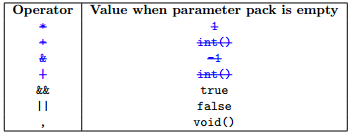
\includegraphics[scale=0.4]{Pictures/table.png}
\caption{\textit{\color{gray}Unary fold expressions. \cite{Bartek}.}}
\end{figure}
\item Remove Deprecated Use of the register Keyword
\begin{lstlisting}
storage-class-specifier:
            register //removed
            static
            thread_local
            extern
            mutable
\end{lstlisting}
\item Remove Deprecated operator++(bool)
\begin{lstlisting}
VQ T& operator++(VQ T&);
T operator++(VQ T&, int);
\end{lstlisting}
\item Removing Deprecated Exception Specifications from C++17
\begin{lstlisting}
void legacy() throw(something) // remove ->throw(something)
try
{
    // function body as before
}
catch(const something&) {
   throw;
}
catch(...) {
   terminate();
}
\end{lstlisting}
\item Make exception specifications part of the type system
\begin{lstlisting}
void (*p)();
void (**pp)() noexcept = &p;   // error: cannot convert 
	to pointer to noexcept function

struct S { typedef void (*p)(); operator p(); };
void (*q)() noexcept = S();   // error: cannot convert 
	to pointer to noexcept function
\end{lstlisting}
\item Aggregate initialization of classes with base classes
\begin{lstlisting}
struct base { int a1, a2; };
struct derived : base { int b1; };

derived d1{{1, 2}, 3};      // full explicit initialization
derived d1{{}, 1};          // the base is value initialized
\end{lstlisting}
\item Lambda capture of *this
\begin{lstlisting}
struct S {
int x ;
void f() {
// The following lambda captures are currently identical
auto a = [&]() { x = 42 ; } // OK: transformed to (*this).x
auto b = [=]() { x = 43 ; } // OK: transformed to (*this).x
a();
assert( x == 42 );
b();
assert( x == 43 );
}
};
\end{lstlisting}
\item Using attribute namespaces without repetition
\begin{lstlisting}
FROM
void f() {
    [[rpr::kernel, rpr::target(cpu,gpu)]] // repetition
    do-task();
}
TO
void f() {
    [[using rpr: kernel, target(cpu,gpu)]]
    do-task();
}
\end{lstlisting}
\item Dynamic memory allocation for over-aligned data
\begin{lstlisting}
class alignas(16) float4 {
    float f[4];
};
float4 *p = new float4[1000];
\end{lstlisting}
\item has include in preprocessor conditionals
\begin{lstlisting}
#if __has_include(<optional>)
#  include <optional>
#  define have_optional 1
#elif __has_include(<experimental/optional>)
#  include <experimental/optional>
#  define have_optional 1
#  define experimental_optional 1
#else
#  define have_optional 0
#endif
\end{lstlisting}
\item Template argument deduction for class templates
\begin{lstlisting}
void f(std::pair<int, char>);

f(std::pair<int, char>(42, 'z'));
\end{lstlisting}
\item Non-type template parameters with auto type
\begin{lstlisting}
template <auto value> void f() { }
f<10>();               // deduces int
\end{lstlisting}
\item Guaranteed copy elision
\begin{lstlisting}
Foo f() {  
    return {};
}

int main() {  
    auto &&foo = f();
}
\end{lstlisting}
\item New specification for inheriting constructors
\begin{lstlisting}
// Inheriting constructor parameters are no longer copied
struct A { A(const A&) = delete; A(int); };
struct B { B(A); void f(A); };
struct C : B { using B::B; using B::f; };
C c({0}); // was ill-formed, now ok (no copy made)
c.f({0}); // ok (unchanged)
\end{lstlisting}
\item Direct-list-initialization of enumerations
\begin{lstlisting}
enum class Handle : uint32_t { Invalid = 0 };
Handle h { 42 }; // OK
\end{lstlisting}
\item Stricter expression evaluation order
\begin{lstlisting}
// unspecified behaviour below!
f(i++, i);

v[i] = i++;

std::map<int, int> m;
m[0] = m.size(); // {{0, 0}} or {{0, 1}} ?
\end{lstlisting}
\item constexpr lambda expressions
\begin{lstlisting}
constexpr auto ID = [] (int n)  { return n; };
constexpr int I = ID(3);
static_assert(I == 3);

constexpr int AddEleven(int n) {
  // Initialization of the 'data member' for n can
  // occur within a constant expression since 'n' is
  // of literal type.
  return [n] { return n + 11; }();
}
static_assert(AddEleven(5) == 16);
\end{lstlisting}
\item Different begin and end types in range-based for
\begin{lstlisting}
From
{
   auto && __range = for-range-initializer;
   for ( auto __begin = begin-expr,
              __end = end-expr;
              __begin != __end;
              ++__begin ) {
        for-range-declaration = *__begin;
        statement
   }
}
To
{
  auto && __range = for-range-initializer;
  auto __begin = begin-expr;
  auto __end = end-expr;
  for ( ; __begin != __end; ++__begin ) {
    for-range-declaration = *__begin;
    statement
  }
}
\end{lstlisting}
\item fallthrough attribute
\begin{lstlisting}
switch (c) {
case 'a':
    f(); // Warning emitted, fallthrough is perhaps 
    a programmer error
case 'b':
    g();
[[fallthrough]]; // Warning suppressed, fallthrough
 is intentional
case 'c':
    h();
}
\end{lstlisting}
\item nodiscard attribute
\begin{lstlisting}
[[nodiscard]] int foo();
void bar() {
    foo(); // Warning emitted, return value of a 
    nodiscard function is discarded
}
\end{lstlisting}
\item maybe unused attribute
\begin{lstlisting}
static void impl1() { ... } // Compilers may warn about this
[[maybe_unused]] static void impl2() { ... } 
					// Warning suppressed


void foo() {
                      int x = 42;
                      // Compilers may warn about this
     [[maybe_unused]] int y = 42; 
     				// Warning suppressed
}
\end{lstlisting}
\item Ignore unknown attributes
\begin{lstlisting}
//compilers which don't support MyCompilerSpecificNamespace
		 will ignore this attribute
[[MyCompilerSpecificNamespace::do_special_thing]]
void foo();
\end{lstlisting}
\item Pack expansions in using-declarations
\begin{lstlisting}
template <typename... Ts>
struct Overloader : Ts... {
    using Ts::operator()...;
    // […]
};
\end{lstlisting}
\item Structured Binding Declarations
\begin{lstlisting}
From
int a = 0;
double b = 0.0;
long c = 0;
std::tie(a, b, c) = tuple; // a, b, c need to be declared first
To
auto [ a, b, c ] = tuple;
\end{lstlisting}
\item init-statements for if and switch
\begin{lstlisting}
if (auto val = GetValue(); condition(val))
    // on success
else
    // on false...
\end{lstlisting}
\item Inline variables
\begin{lstlisting}
struct MyClass
{
    inline static const int sValue = 777;
};
\end{lstlisting}
\item DR: Matching of template template-arguments excludes compatible templates
\begin{lstlisting}
template <template <typename> typename Container>
struct A
{
    Container<int>    m_ints;
    Container<double> m_doubles;
};
\end{lstlisting}
\item std uncaught exceptions()
\begin{lstlisting}
int uncaught_exceptions() noexcept;
\end{lstlisting}
\item constexpr if-statements
\begin{lstlisting}
template <typename T>
auto get_value(T t) {
     if constexpr (std::is_arithmetic_v<T>) {
         //...
     }
     else {
         //...
     }
}
\end{lstlisting}




\end{enumerate}

}


\subsection{C++ Libraries}
The C++ Object Oriented Programming language including a Standard Library what is a collection of classes and functions and the Standard Function Library that are inherited of C and part of the C++ ISO standard.\cite{Tutorialspointlibraries}\\

The Standard Libraries provide several interface to manipulate data, function objects, string, data structures through specific syntax and semantics of generics algorithms to the C++ programming language for daily task like find the fraction of a number, printing to the screen, threaded programming, iterations and much more.\\ \cite{Tutorialspoint}

\begin{enumerate}
\item Standard Function Library : General purpose, stand-alone functions and not part of nay class.
	\begin{itemize}
	\item I/O
	\item String and character handling,
	\item Mathematical,
	\item Time, date, and localization,
	\item Dynamic allocation,
	\item Miscellaneous,
	\item Wide-character functions,
	\end{itemize}
\item Object Oriented Class Libraries : Collection of Classes and inherited functions.
	\begin{itemize}
	\item The Standard C++ I/O Classes,
		\begin{itemize}
		\item iosfwd
		\item ios
		\item istream
		\item iostream
		\item ostream
		\item fstream
		\item sstream
		\item strstream
		\item iomanip
		\item streambuf
		\item cstdio
		\end{itemize}
		
	\item Thread Support libraries,
		\begin{itemize}
		\item thread
		\item mutex
		\item shared mutex
		\item future
		\item condition variable
		\end{itemize}
		
	\item Atomic operation library,
		\begin{itemize}
		\item atomic
		\end{itemize}
	\item Filesystem library,
		\begin{itemize}
		\item filesystem
		\end{itemize}
		
	\item Regular Expression library,
		\begin{itemize}
		\item regex
		\end{itemize}
		
	\item Localization library,
		\begin{itemize}
		\item locale
		\item clocale
		\item codecvt
		\end{itemize}
		
	\item The String Class,
		\begin{itemize}
		\item cctype
		\item cwctype
		\item cstring
		\item cwchar
		\item cucchar
		\item string
		\item string view
		\item charconv
		\end{itemize}
		
	\item The Numeric Classes,
		\begin{itemize}
		\item cmath
		\item complex
		\item valarray
		\item random
		\item numeric
		\item ratio
		\item cfenv
		\end{itemize}
		
	\item The STL Container Classes,
		\begin{itemize}
		\item array
		\item vector
		\item deque
		\item list
		\item forward list
		\item set
		\item map
		\item unordered list
		\item unordered map
		\item  stack
		\item  queue
		\end{itemize}
		
	\item The STL Algorithms,
		\begin{itemize}
		\item algirithm
		\item execution
		\end{itemize}

	\item The STL Iterators,
		\begin{itemize}
		\item iterator
		\end{itemize}
		
	\item The Localization library,
		\begin{itemize}
		\item locale
		\item clocale
		\item codecvt
		\end{itemize}
		
	\item Exception Handling Classes,
		\begin{itemize}
		\item execption
		\item stdexcept
		\item cassert
		\item system error
		\item cerno
		\end{itemize}
		
	\item Dinamic memory management,
		\begin{itemize}
		\item new
		\item memory
		\item scoped allocator
		\item memory resource		
		\end{itemize}
		
	\item Utilities library
		\begin{itemize}
		\item cstdlib
		\item csingnal
		\item csetjmp
		\item cstdarg
		\item typeinfo
		\item typedindex
		\item typed traids
		\item bitset
		\item functional
		\item utility
		\item ctime
		\item chrono
		\item cstddef
		\item initalizer list
		\item tuple
		\item any
		\item optional
		\item variant
		\end{itemize}
		
	\end{itemize}
\end{enumerate}







\clearpage
\section{Platforms}
C++ is a compiled language while some other programming language is interpreted. It means the C++ code can not run directly from the Integrated Development Environment(IDE) it need to invoke the compiler to to generate an executable that can run on the operating system. This executable can run only the operating system platform in which compiler created the executable file. However, the C++ programming language is cross-platform, it means able to run on all operating system but the executable can run only the type operating system platform where it was created. It is also possible to create a semi-complied C++ code use the LLVM compiler to produce LLVM byte code, and them the target operating system platform can completing the translation from byte-code to the final executable file. So. to run the C++ code on different platform the code must be complied with the target platform to run on it. \cite{G2}\\ 

{\setlength{\parindent}{0cm} 
\textbf{The main platforms for desktop computer are:}
}
\begin{enumerate}
\item Mac OsX //derived from Unix
\item Windows
\item Linux // Kernel
	\begin{enumerate}
	\item Ubuntu
	\item Debian
	\item Red hat
	\item Fedore
	\item Suse
	\end{enumerate}
\item Solaris //derived form Unix
\item Unix systems
	\begin{enumerate}
	\item FreeBSD
	\item NetBSD
	\item OpenBSD
	\end{enumerate}
\item Amiga
\item OpenVMS
\item Mobile phone platforms //iOS, Android, Blackberry etc..
\end{enumerate}

\subsection{Integrated Development Environment(IDE)}
IDE is a software product that provide comprehensive set of tools to programmers to create software products in different programming languages. 
To create an application in any programming language the best way to use an IDE. The IDE give a suggestions for programming language syntax, highlights errors, matching brackets and can run a source code with the built in runtime environment. The another very useful function is a built in debugger in the IDE. To find logical errors in the code more difficult then find syntax errors. Some of the IDE has no default debugger built in, then need to attach a remote debugger to the IDE.\\

Some of the IDE are supporting many programming languages, some of them specialized only for one given language. Most of the IDE are cross-platform but some are written for single-platform. There are many IDE available but here will be describe only few of the top IDE developer tools.\\
{\setlength{\parindent}{0cm}
\begin{enumerate}
\item \textbf{QT creator : }is available for free with free core libraries or payable professional libraries as well. \textit{"Qt Creator provides a cross-platform, complete integrated development environment (IDE) for application developers to create applications for multiple desktop, embedded, and mobile device platforms, such as Android and iOS."}\cite{QT} It is supported on variety of 64 and 32-bit systems with the built in GCC vendor supplied compiler, or can attach any third party compiler. Qt provide code editor with C++, QML and ECMAscript, syntax highlighting and code completion, static code checking, source code refactoring and parenthesis matching.The most powerful feature is the Qt GUI application development framework that includes integrated GIU designer. QT use has it is own GUI libraries to place C++ Qt widgets to create visual applications.\\

QT creator has integrated set of tool like version control to connect with:
\begin{enumerate}
\item Git
\item Subversion
\item Perforce
\item CVS
\item Mercurial
\end{enumerate}

It does not include  a debugger for native code, but it provide debugger plug-in that acts interface between the IDE and the external debugger to debug C++ code. Supported debuggers are :
\begin{enumerate}
\item GNU debugger (GDB)
\item LLVM debugger (LLDB)
\item Microsoft Console Debugger (CDB)
\item Internal Javascript Debugger
\end{enumerate}

Supported platforms : 
\begin{enumerate}
\item Linux
\item Windows
\item MacOS
\end{enumerate}

\item \textbf{Microsoft Visual Studio(MSVS) : } is Microsoft IDE that available in free community version and payable professional version. MVSV is a very powerful software developer kit to create desktop, web, mobile, console and nearly any kind of application. It's code editor support IntelliSense(code completition) and code refactoring. MSVS has built integrated debugger that works on source-code and on machine-code level as well. As a built in feature MSVS able to create C++ GUI application without any external library. However, it is works on Windows platform and just released to Mac OsX, Microsoft Visual Studio is a very powerful Integrated Development Environment.\cite{VS}\\

Microsoft C and C++ compiler and linker is the cl.exe that produce the Common Object File Format(COFF), objetc file (.obj) and produce the executable (.exe)file or dynamic-link(Dlls) libraries. 

MSVS has built in version control and can connect to different version control systems:
\begin{enumerate}
\item Git
\item GitHub
\item AnkhSVN
\item Team Foundation Version Control(TFVC)
\item other extensions
\end{enumerate} 

Supported platforms : 
\begin{enumerate}
\item Windows
\item MacOS from 2017
\end{enumerate}

\item \textbf{Netbeans : } is a free IDE provide developer interface for many different languages. Netbeans provide project types and templates for C and C++ projects. It is well integrated with GNU gdb debugger, code refactoring, code completiton. Supports variety of leading compiler such Oracle Solaris Studio, GNU, CLang, LLVM, Cygwin, MinGW, and has option to pre-process definition, compile-time, language standards etc. As an interesting factor in Netbeans support QT application development framework to create GUI application.\cite{Netbeans}\\

Netbeans provide version control in default for some remote system:
\begin{enumerate}
\item Git
\item Mercurial
\item Subversion
\item other extensions/plugins are available to connect to different version control systems.
\end{enumerate} 

Supported platforms : 
\begin{enumerate}
\item Linux
\item Windows
\item MacOS
\end{enumerate}

\item \textbf{EMACS : } is a free extensible, customizable, self-documenting, real-time display free text editor. It is a highly customizable developer kit since it has more than 10,000 built-in commands, that the user can combine and automatize to do automated work. Use Lips programming language in the background to operate the IDE. Since Emacs use its own key combination, thus the users who never used before Emacs, it could be very difficult at the begging. Supporting lots of different programming languages, other text and unicode format as well. Since Emacs use command line to control the IDE and compile the C++ code, thus any type of compiler can be use with it.\cite{Emacs}\\

Emacs version control interface is called VC. Commands works with several different version control systems:
\begin{enumerate}
\item Bazaar
\item CVS
\item Git
\item Mercurial
\item Monotone
\item RCS
\item SCCS/CSSC
\item Subversion
\end{enumerate} 

Supported platforms : 
\begin{enumerate}
\item Linux
\item Windows
\item MacOS
\end{enumerate}

\end{enumerate}
}

\subsection{Compilers}
While the IDE helps to create a runnable code the compiler takes this program code or source code/high-level language and converts it to machine code or low-level language. Then that code will be translated to an executable file that the computer able to run on the operating system. In other word, the compiler converts the instructions set to machine code that computer can run. The different platforms has many different free and payable compilers available to use. There are  major different between the compilers like code optimization, minor syntactical difference, runtime libraries used, header, implementation and more.\cite{Bolton}\\

To create a cross-platform project in C++ has no real solution. The best way to run a C++ application on the target platform is to use the default platform supported or a platform specific compiler.\\

\textit{"CMake is an extensible, open-source system that manages the build process in an operating system and in a compiler-independent manner."\cite{CMake}} Every platform needs to have some sort of file that build the required program from the source code in a manner to linking the files in the project and creating the output files. On Unix/Linux system the Make file is responsible for this task. If we want to build the same source code on Microsoft Windows platform, then need a different make file called nmake.\\

 Make is a build-system that drives the compiler and the build tools to build the application from the source code. CMake is a generator for build-system. it can produce platform specific build files using the CMakeList.txt file.\\

{\setlength{\parindent}{0cm}
Many compilers available in the market for different purpose and platforms. In the following list can find the main compilers with short description:\cite{Heng} 
\begin{enumerate}
\item GCC\\
Part of the GNU compiler Collection and the standard compiler for Unix-like operating systems and the C programming language. 
\item G++\\
Part of the GNU compiler Collection is same as the GCC but extended to compile the C++ programming language.
\item MVSC\\
Microsoft Visual C++ IDE with built in compiler for Microsoft operating system to create Windows API, .NET framework and much more.
\item Clang\\
Is the default compiler for Mac OS development it replaced the GCC compiler in 2005.
\item MinGW-w64\\
Provide Libraries and header to the GNU compiler to run on Windows system.
\item AMD x86 Open64\\
Is a version of Open64 compiler that has been used for AMD processors.
\item OrangeC\\
Supports C standars like C99 and C11, and it is runs on Windows and DOS.
\item Apple Xcode\\
Is an Apple IDE with built in GNU C compiler.
\item TinyC\\
Is a small Linux and Windows compiler that generates x86 native binaries.
\end{enumerate}
}
\subsubsection{GCC and G++}
The GCC and G++ programs are not compilers, but drivers that can invoke other other programs depending on the arguments that passing with it in the terminal. The programs that GCC and G++ invokes with the argument can be such as cp compilers and cc1 linkers, ld assembler which are part of the GNU Compiler Collection. So, GCC use the C compiler and the G++ use the C++ compiler\cite{Rohan} 

\subsubsection{MVSC}
MSVC in an IDE for Microsoft system, that include compiler, debugger, editor and profiler. MVSC compiler supports most of ISO C++11 most of C++14 and C++17, while the C compiler is outdated. Provide support for diverse languages to create applications for Windows desktop and mobile, Andriod platform to compile and run.\cite{Heng}\\

\subsubsection{CLANG}
Clang is a compiler developed by Apple and support C,C++, Objective C and Objective C++ languages. It is part of the Low Level Virtual Machine(LLVM) project and intermediate compiler language for LLVM IR what is provide instruction that similar output like the byte code. The back end of LLVM generates the machine code for the targeted system and required processor. The idea of CLang to mix the compiler front end with the targeted back-end. The front end compiler support many languages.\cite{BoltonD}

\subsection{Conclusion of platform}
All of the computing platforms providing compiler solution not only for C and C++ programming languages but all the programming languages that are able to run on the operating system. However, the compilers are around since decades but is still no real cross-platform compiler solution for the C programming language family. If the source code written in the plain C99 or C++11 standard without any external library that should able to compile on any Unix-based standard operation system platform but not on Windows. To get working on Windows platform need to use conditional compilation with \#if preprocessor directive to wrap all the operating specific services at compilation time.\\ 

Qt development is a cross platform GUI builder to create C++ application that can run on any targeted platform if the required libraries are installed in the target operation system. Qt uses the vendor system GCC compiler or third party attached compiler.

\clearpage
\section{Conclusion}

\subsection{Concurrency as a base problem}
The parallel programming pattern has many advantages, but as any other programming design it has disadvantages as well. The concurrent and parallel programming design help the application to handle multitasking and are able to speed up the the software execution time. While a user executes multiple instructions within the application in the background, the software breaks down the instructions to parallel to the CPU cores and creates threads to handle computations in a faster manner than the sequential programming design.\\ 

As advantages in concurrent programming design  is to help increase the performance, the reaction time of the applications and parallel programming fashion maximizes the CPU throughput in efficient manner. 

However, it has lots of advantages that must mention the difficulties with the code writing design and the complicated debugging process as the disadvantages.   

\subsection{Software Transactional Memory}
The Software Transactional Memory is a lock free solution of concurrent programming, since it doesn't need to use mutex and semaphores to control threads. It is easier to read , maintain, extend and work with the high level objects and modules. It offers transactional environment without extra hardware cost.\\ 

As the main advantages the STM prevents deadlock, livelock, uses transactional methods, atomic variables and controlling the threads in easier manner than the semaphores and mutex can. As a disadvantage, performance issues can happen because the transactions may roll back too many times before the threads finish their execution in the transactional function.\\

\subsection{Platform and Compilers}
C and C++ programming languages are required compiler to translate the source code to object code or machine code to run on the operating system. Every programming language has many different versions of compiler on the different operating platforms. However, there are many compiler forms in  diverse languages, no real cross-platform compiler solution to the C programming language family. If the source code is written in the plain C99 or C++11 standard without any external library, that should be able to compile on any Unix standard operation system platform but not on Windows. To get working on Windows platform, it needs to use conditional compilation with \#if preprocessor directive to wrap all the operating specific services at compilation time.\\ 

QT development is including the QT libraries and the GUI designer to create cross platform C++ applications that can run on any targeted platform, if the build process doesn't include any other libraries that comes outside of the QT framework. QT uses the vendor system GCC compiler or third party attached compiler to create the machine code.

\newpage
\section{Bibliography}
\begin{center}
\bibliographystyle{siam}
\bibliography{database.bib}

\end{center}


\end{document}